Before delving into gradients and their pivotal role in deep learning, let us briefly revisit a fundamental concept from calculus, the {\em derivative}. At its core, the derivative provides us with a measure of how a function $f: {\mathbb R} \to {\mathbb R}$ changes as its input varies. Represented by \( \frac{df}{du} \), the derivative signifies the slope of the tangent line to the function's curve at a specific point $u \in {\mathbb R}$. The derivative can also be seen as a function, $f':{\mathbb R} \to {\mathbb R}$, where $f'(u)$ is the derivative at a specific point $u$, namely $f'(u) = \frac{df}{du}$.  

An estimate of the slope of the function (rise divided by run) at a specific point $u$ is
%
\[
\frac{\textrm{Rise}}{\textrm{Run}} = \frac{f(u+\Delta) - f(u)}{(u+\Delta) - u} = \frac{f(u+\Delta) - f(u)}{\Delta},  
\]
%
where $\Delta$ is a positive small number such that $u$, and $u + \Delta$ are two nearby points on ${\mathbb R
}$. We can then treat the derivative of $f(~)$ at $u$ as the limit of this slope as $\Delta$ gets small. Formally one can write this as,
%
\[
f'(u) = \lim_{\Delta \to 0} \frac{f(u+\Delta) - f(u)}{\Delta}.
\]
%
A deeper understanding of derivatives may require a review of basic {\em calculus} which we cannot afford in this exposition. For this, we refer the reader to any basic calculus text, or online resource. One interesting and enjoyable read which may help readers gain insight on this topic is {\em Burn Math Class: And Reinvent Mathematics for Yourself} \cite{wilkes2016burn}.

In deep learning we use derivatives for training. Consider first an hypothetical scenario where we are training a model with a single parameter $\theta$. Now as denoted at the end of Section~\ref{sec:sets-and-functions}, we have a loss function $C_{\textrm{Data}}(\theta)$, and we wish to minimize this function. For this we can use the derivative $\frac{dC}{d\theta}$ to gain information about the slope of the function, and this gives us an indication about the directions and the magnitudes that can be used in our optimization procedure. Ultimately, with the aid of derivatives, we try to find the best $\theta$ for the loss. Note that in this section we denote $C$ as shorthand for $C_{\textrm{Data}}$.

Now, let us extend our perspective to a more complex scenario where our model has multiple parameters, often denoted as $\theta = (\theta_1, \theta_2, ..., \theta_d)$, similarly to the presentation at the end of Section~\ref{sec:sets-and-functions}. If we are in Model~I then these $d$ parameters are $b_0$ and the $p$ elements of the vector $w$, so $d=p+1$. If we are in Model~II then those $d$ parameters can be taken as the vector $b \in {\mathbb R}^K$ and the matrix $W \in {\mathbb R}^{K\times p}$, so the vector $\theta$ is of dimension $d = p + pK = p(K+1)$. If we are in Model~III then $\theta$ is even more complex and constitutes the weights and biases in all layers; details for Model~III are in the next section. In any case, we treat all the individual parameters in the vectors and matrices as one long vector $\theta$ with $d$ elements.  

We now generalize the notion of the derivative from one dimension to $d$ dimensions using the notion of a {\em gradient}. For a parameter point $\theta \in {\mathbb R}^d$, the gradient denoted as $\nabla C(\theta)$ is a vector in ${\mathbb R}^d$ which points at the direction of steepest ascent and has a magnitude (norm) which captures how steep the function is in that direction. In fact, the gradient is composed of individual partial derivatives, and $\nabla C(\theta) =  \left(\frac{\partial C}{\partial \theta_1}, \frac{\partial C}{\partial \theta_2}, ..., \frac{\partial C}{\partial \theta_d}\right)$. Note that each partial derivative $\frac{\partial C}{\partial \theta_j}$ is the derivative of $C(\theta)$ with respect to $\theta_j$ assuming that all other parameters are fixed. Just like the derivative which can be viewed as a function, the gradient can also be viewed as a function,
%
\begin{equation}
\label{eq:grad-def}
\nabla C: {\mathbb R}^d \to {\mathbb R}^d.
\end{equation}
%
For loss functions $C(~)$ with vector inputs of length 2 as illustrated in Figure~\ref{fig:GD-LR-SR}, the gradient can be drawn as an arrow on the plane. For loss functions with vector inputs of length 3, the gradient is an arrow in 3 dimensional space. For loss functions of higher dimensions (it is common in deep learning to have $d$ in the order of millions or more), we as humans cannot visualize the gradient, yet it describes the direction of movement of steepest ascent/increase. 

Importantly, when we consider loss landscapes for deep learning, the gradient tells us the slope of the terrain and points us in the direction where the loss increases most rapidly. Imagine standing at a point on this landscape where the direction we would move to ascend the slope most rapidly is precisely the direction of steepest increase. However, our goal is to descend into the valleys, seeking the lowest points where the loss is minimized. To achieve this, we utilize the negative of the gradient (scalar multiplication of the gradient by $-1$), as it points in the direction of steepest decrease. In fact we further multiply the gradient by the scalar $\alpha$, called the {\em learning rate}, which controls how big of a step we take.

During the training of a deep learning model, our objective is to iteratively adjust the model's parameters in the opposite direction of the gradient. This process, known as {\em gradient descent}, guides us downhill, helping us reduce our loss in the loss landscape. The key idea is to use an update such as,
%
\begin{equation}
\label{eq:gdls1}
\theta^{(t+1)} = \theta^{(t)} - \alpha \nabla C(\theta^{(t)}),
\qquad
\text{with}
\qquad
\alpha > 0,
\end{equation}
%
where $\theta^{(t)}$ is the current parameter point and $\theta^{(t+1)}$ is the next parameter point. We start at some initial guess  $\theta^{(0)}$ then iterate via \eqref{eq:gdls1} to improve our parameters; namely to train our model. The learning rate, $\alpha$,  specifies how big of steps we take during the algorithm. The learning rate is an example of an {\em hyper-parameter} in deep learning and it sometimes requires tweaking for gradient descent to work well.

As an algorithm, using a sequence of steps which one may convert to code in a programming language such as Python, R, or Julia, we may specify this basic gradient descent algorithm with {\em pseudo code}. In particular these are the  steps of the algorithm:

\vspace{0.5cm}
% %
\begin{algorithm}[H]
\renewcommand{\thealgocf}{} % Remove numbering for this algorithm
\DontPrintSemicolon
  $\theta \leftarrow \theta^{(0)}$
  
  \Repeat{$\theta$ \normalfont{satisfies a} \em{termination condition}} { 
  Compute the gradient $ \nabla C(\theta)$\\
   $\theta \leftarrow \theta - \alpha \nabla C(\theta)$
  }
%   \Return $\theta$
\caption{Gradient descent with loss $C(\theta)$}\label{alg:basic-gradient-descent}
\end{algorithm}
% %
\vspace{0.5cm}

%
Note that the use of expressions such as $a \leftarrow b$ in steps 1 and 4, imply to substitute the value of the right hand side $b$ into the left hand variable $a$. With an algorithm as specified above, the parameters of the model $\theta$ are in memory at all times, and as the algorithm iterates over steps 2 -- 5, these parameters are updated at each time when step 4 is executed. Observe that this step implements the update in \eqref{eq:gdls1}. After the algorithm starts with an initial guess $\theta^{(0)}$ (step 1), each iteration of steps 2 -- 5 yield a new update, where in the first iteration we have $\theta^{(1)} = \theta^{(0)} - \alpha \nabla C(\theta^{(0)})$, in the second iteration we have $\theta^{(2)} = \theta^{(1)} - \alpha \nabla C(\theta^{(1)})$, and so fourth. Note that in this specification we do not go into the termination condition of step 5. See Chapter~4 of  \cite{LiquetMokaNazarathy2024DeepLearning} for more details about this gradient descent algorithm and its generalizations and variants, and in particular the most popular variant for deep learning called ADAM, \cite{kingma2014adam}. 

Importantly, we should mention that step~3 computes the gradient in each iteration, and hence this step can be computationally intensive for large deep learning models. Simple models such as our Model~I and Model~II actually have closed form formulas for the gradient, but for cases such as Model~III, this is where the famous {\em backpropagation algorithm} is used. Namely, the  execution of step~3 is actually the result of running a whole other algorithm based on ideas called {\em backward mode automatic differentiation}. Details of backpropagation are studied in chapters 4 and 5 of \cite{LiquetMokaNazarathy2024DeepLearning}.

\begin{figure}[h!] 
  \begin{subfigure}[b]{0.5\linewidth}
    \centering
    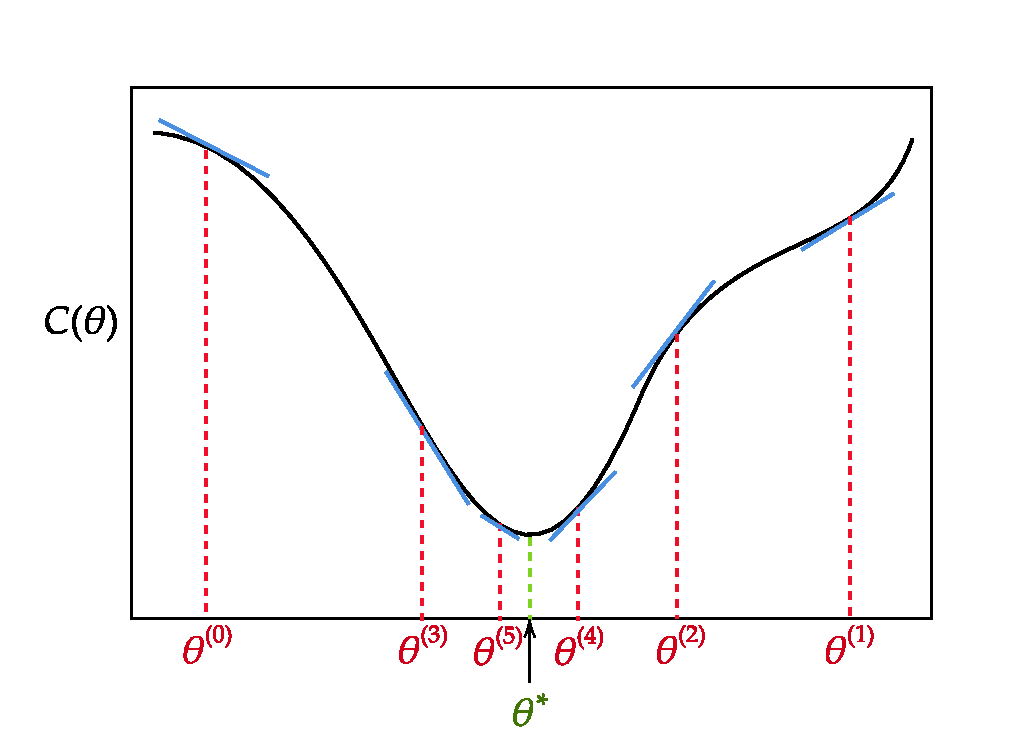
\includegraphics[width=0.99\linewidth, height=0.8\textwidth, trim=20 20 20 20]{../supporting_files/figures/GD_1d.pdf}
    \caption{} 
    \vspace{2ex}
  \end{subfigure}%% 
  ~
  \begin{subfigure}[b]{0.5\linewidth}
    \centering
    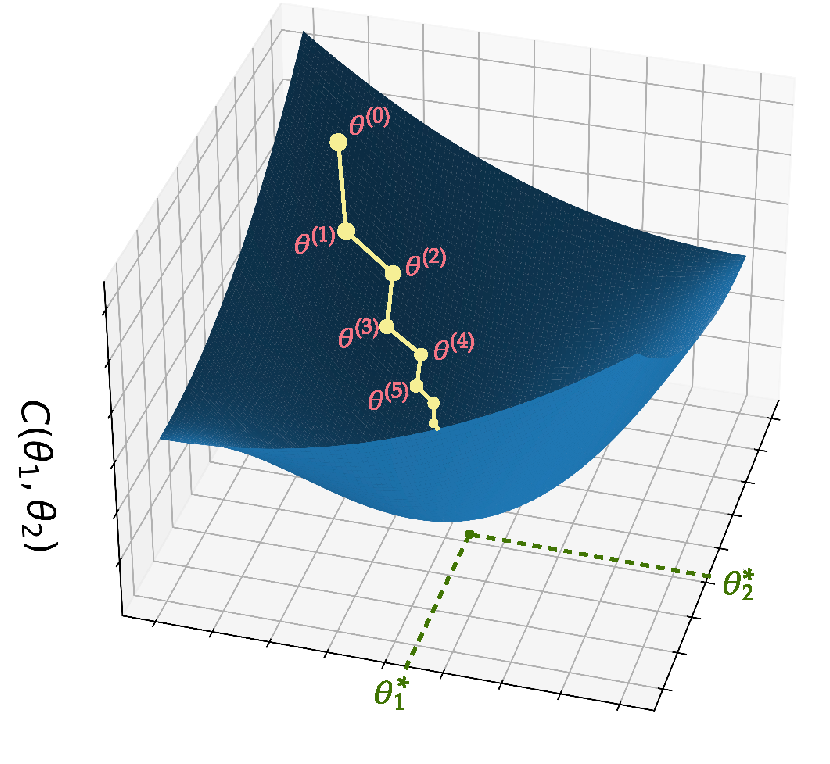
\includegraphics[width=0.9\linewidth, trim=20 20 20 20]{../supporting_files/figures/GD_2d.pdf}
    \caption{} 
    \vspace{2ex}
  \end{subfigure} 
    \caption{Illustration of gradient descent for 5 iterations starting with $\theta^{(0)}$ and getting near the optimum $\theta^*$ with $\theta^{(5)}$. (a)~A one-dimensional loss landscape $C(\theta)$ with $\theta \in \mathbb{R}$. (b)~a two-dimensional loss landscape $C(\theta_1,\theta_2)$ with $\theta = (\theta_1, \theta_2) \in \mathbb{R}^2$.}
    \label{simpleloss}
\end{figure}

As an illustration of gradient descent, see Figure~\ref{simpleloss}. First in (a) we consider a  model with a single parameter $\theta \in \mathbb{R}$ and the associated loss function $C(\theta)$ plotted with a minimum at $\theta^*$.  The gradient descent algorithm starts with an initial guess $\theta^{(0)}$ and then updates to $\theta^{(1)}$ using $\theta^{(1)} = \theta^{(0)} - \alpha \nabla C(\theta^{(0)})$. In this simple one dimensional case, the gradient at the point $\theta^{(0)}$ reduces to the derivative, $C'(\theta_0)$, which is the slope of the tangent at the point $\theta^{(0)}$. In our example this derivative is negative, then by multiplying this derivative by $-\alpha$ we move in the opposite direction (right) than the gradient. Using the same process, the next move is driven by $\theta^{(2)} = \theta^{(1)} - \alpha  C'(\theta^{(1)})$. Note that in this case the slope of the tangent at the point $\theta^{(1)}$ is positive. Then by multiplying by $- \alpha $, we are move left towards the minimum. In the figure we show the iterates up to $\theta^{(5)}$ which is not far from the minimal point $\theta^*$.

In Figure~\ref{simpleloss}~(b) we see a similar trajectory, only this time moving on the $(\theta_1, \theta_2)$ plane, and the points are plotted on the surface as $C(\theta^{(i)})$. Here in this example, small steps move in the direction of steepest descent, ultimately reaching a point close to the optimum $\theta^* = (\theta_1^*, \theta_2^*)$. The reader should comprehend that with realistic problems, the number of parameters $d$ can be in the order of millions. Hence each gradient descent iteration is a step in such a high dimensional space, which we cannot visualize. 
